\section{Introduction}
\label{sec:introduction}

Magic squares are among the oldest objects of recreational mathematics: the $3\times3$ Lo Shu belongs to Chinese tradition, a $4\times4$ square is engraved in Albrecht D\"urer's \emph{Melencolia~I} (1514) alongside a balance scale and a $12$-vertex convex polyhedron (\emph{D\"urer's solid}, a truncated rhombohedron), and constructions for every order $n\ge3$ have been known for centuries \cite{andrews1960magic,pickover2002zen}.
The modern literature treats them from several directions: enumeration and the geometry of the polytopes whose lattice points are the squares \cite{stanley1973magic,ehrhart1973magic,ahmed2003polyhedral,beck2006insideout,beck2010enumeration}, spectral and matrix properties \cite{loly2009spectra,nordgren2012properties,nordgren2014spectra,cameron2013signatura}, and, in work of Loly and collaborators, physical invariants such as the moment of inertia and the multipole moments \cite{loly2004invariance,rogers2004inertia,rogers2005multipole}.
Magic squares have also been read as height fields: Knecht's water-retention problem asks how much water a magic square of order $n$ can hold when its entries are the heights of the cells \cite{oeis_A201126}, and led to the study of water retention on random surfaces \cite{knecht2012retention}.

\begin{definition}[Magic square]
\label{def:magic_square}
An \emph{arrangement} of order $n$ is a bijection $S=(s_{ij})$ from the cells of the $n\times n$ grid onto $\{1,\dots,n^2\}$ (a permutation of $1,\dots,n^2$ written into the grid).
It is a \emph{magic square} if every row, every column and both main diagonals sum to the magic constant $\mu_n=n(n^2+1)/2$, and \emph{semi-magic} if only the rows and columns do.
\end{definition}

\paragraph{The construction.}
Centre the grid at the origin and attach to the cell $(i,j)$ of an arrangement the point
\[
\mathbf p_{ij}=(x_{ij},y_{ij},z_{ij}),
\]
whose horizontal part $(x_{ij},y_{ij})$ is the position of the cell and whose height $z_{ij}=s_{ij}-\frac{n^2+1}{2}$ is the entry minus the mean entry.
The \emph{gem} $\mathcal G(S)$ is the convex hull of these $n^2$ points (\Cref{sec:gem}).
It is defined for every arrangement: the points are the lift of a fixed grid by a permutation of fixed heights, and the lower and upper faces of the gem are the regular subdivisions $\mathcal S(z)$ and $\mathcal S(-z)$ of the grid, glued along its boundary (\Cref{prop:subdivisions}).
Magic squares are the motivating case, and we call the gem of a magic square a \emph{Magic Gem}: read as vectors from the origin, its points have vertical components that cancel along every row, column and both diagonals (\Cref{lem:lines}; Figures~\ref{fig:vectors} and~\ref{fig:lines}).
Uniting the three emblems of \emph{Melencolia~I}, the equal row and column sums place the lifted heights in mechanical balance about the origin, and the gem of D\"urer's square is itself a centrally symmetric $12$-vertex polyhedron with $f$-vector $(12,24,14)$ and $4$ interior points (\Cref{fig:vectors}).

\begin{figure}[htbp]
\centering
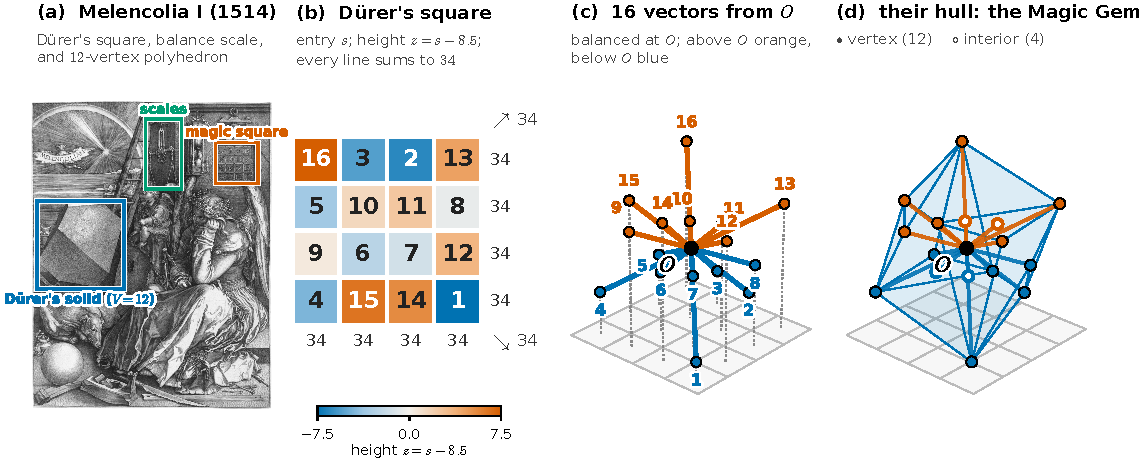
\includegraphics[width=0.98\textwidth]{figures/fig_vectors.pdf}
\caption{From \emph{Melencolia~I} to the Magic Gem. (a)~Albrecht D\"urer's engraving \emph{Melencolia~I} (1514, public domain), highlighting the $4\times4$ magic square, the balance scale, and D\"urer's $12$-vertex truncated rhombohedron ($f=(12,18,8)$). (b)~D\"urer's square with entries $s_{ij}$ on a heat map of the heights $z_{ij}=s_{ij}-8.5$ (orange above $0$, blue below); every line sums to $34$. (c)~The $16$ vectors $\mathbf p_{ij}$ from the origin $O$, labelled by the entries, with drop lines to the floor grid. (d)~Their convex hull, the Magic Gem ($f=(12,24,14)$): $12$ tips are vertices (filled) and $4$ lie in the interior (open). The colour bar is shared by (b) and (c).}
\label{fig:vectors}
\end{figure}

\paragraph{Results.}
The main result is a theorem about one classical family.
\emph{For the Siamese (de la Loub\`ere) square of every odd order $n\ge5$ the vertices of the gem are exactly the twelve points that the boundary of the grid forces (the corners and, on each side, the cells of the smallest and the largest entry); the $f$-vector is $(12,26,16)$ and the isometry group is $\{\pm\mathrm{id}\}$} (\Cref{thm:siamese}).
So only $12$ of the $n^2$ points are vertices, whereas the gems of random arrangements and of sampled magic squares have more and more vertices as $n$ grows (\Cref{tab:vertices}, estimates).
The proof shears the lift onto five levels and reduces to the signs of a table of polynomials in $m=(n-1)/2$.
The same method shows that the square with the two base-$n$ digits exchanged has a gem with $f$-vector $(12,24,14)$ for every odd $n\ge5$ (\Cref{prop:exchanged}); along the way we give a self-contained criterion for a linear square (a square of the uniform step method) to be magic, and count these squares (\Cref{prop:linear-magic}).
More generally, along every family of linear squares with fixed steps and offsets affine in $n$ the vertex count is bounded and the $f$-vector is eventually periodic in $n$ (\Cref{prop:fixed-steps}).
The bound depends on the family: over all linear magic squares of prime order $n$ the largest vertex count grows like $\Theta(\ln n)$ and is at least $\lceil\ln n/(4\ln\varphi)\rceil+2$, with $\varphi$ the golden ratio (\Cref{cor:many-vertices}), and, by computation, for $7\le n\le21$ the Siamese and the digit-exchanged squares are the only linear magic squares, up to $D_4$, with as few as twelve vertices (\Cref{rem:linear}).

The other results require weaker hypotheses than the full magic conditions, and several hold for every arrangement; \Cref{tab:hypotheses} lists what each result needs.
The lifted points balance about the origin for every arrangement, and the heights balance as weights on the grid if and only if the rows and columns have equal sums (\Cref{sec:balance}).
When only the first moments $\sum z\,x$ and $\sum z\,y$ of the heights vanish, the second-moment matrix of the point set is $\operatorname{diag}(a_n,a_n,b_n)$ with $a_n\ne b_n$, and a four-line principal-axes argument shows that the point set has a non-trivial isometry if and only if the arrangement equals its complement up to $D_4$ (\Cref{prop:pointset}).
For the $880$ magic squares of order four up to rotation and reflection we compute all gems in exact integer arithmetic: the isometry group of each gem equals that of its point set, so $48$ gems are centrally symmetric, $304$ have a single half-turn symmetry and $528$ have trivial symmetry (\Cref{prop:iso4}). Across the $880$ squares, the gems have between $8$ and $16$ vertices, realizing $39$ distinct $f$-vectors, $352$ combinatorial types, $155$ exact volumes and $616$ congruence classes (\Cref{prop:congruence}); moreover, the vertex set alone uniquely determines the magic square, for $871$ of the $880$ classes already from the rank of the line-sum equations on the non-vertex cells (\Cref{rem:vertexset}).

Finally, \Cref{sec:magic-vs-random} compares magic gems with the gems of semi-magic squares, of arrangements with vanishing first moments and of random arrangements: whereas combinatorial counts such as the mean numbers of vertices and facets are nearly unchanged across these families, continuous invariants—specifically the volume and the solid centroid—shift systematically as the line-sum constraints are imposed.

\begin{table}[htbp]
\centering
\caption{The results and the hypotheses they need. $^*$Except the eight $D_4$-images of the natural square $s_{ij}=ni+j+1$, whose points are coplanar.}
\label{tab:hypotheses}
\footnotesize
\setlength{\tabcolsep}{4pt}
\begin{tabular}{l l l}
\toprule
result & statement & hypothesis\\
\midrule
\Cref{lem:lines}, \Cref{lem:forced}, \Cref{lem:selfcomp} & centring; forced vertices; complements & any arrangement\\
\Cref{prop:fulldim}, \Cref{prop:subdivisions} & $3$-polytope; faces $\mathcal S(z)$, $\mathcal S(-z)$ & any arrangement$^*$\\
\Cref{lem:cov}, \Cref{prop:pointset} & second moments; point-set isometries & vanishing first moments\\
\Cref{lem:parity} & parity of $V$, $V^\partial$, $V^\circ$; of $E$, $F$ & self-complementary$^*$; associative$^*$\\
\Cref{prop:iso4}, \ref{prop:congruence}, \Cref{rem:vertexset} & order-four census & magic, $n=4$ (computation)\\
\Cref{sec:magic-vs-random} & which invariants see the line conditions & $n=4,5$ (computation)\\
\Cref{prop:linear-magic} & magic linear squares & linear squares, odd $n$\\
\Cref{thm:siamese}, \Cref{prop:exchanged} & Siamese and digit-exchanged gems & two magic squares, odd $n\ge5$\\
\Cref{prop:fixed-steps}, \Cref{cor:many-vertices} & fixed steps; largest vertex count & linear squares; prime $n$\\
\bottomrule
\end{tabular}
\end{table}

\paragraph{Relation to previous work.}
In polyhedral combinatorics, one traditionally studies the space of \emph{all} magic squares of order $n$ simultaneously: nonnegative integer matrices with line sums equal to $t$ are the lattice points of the $t$-th dilate of the Birkhoff polytope \cite{stanley1973magic,ehrhart1973magic,ziegler1995lectures}, magic squares with distinct entries are counted by Ehrhart quasi-polynomials of inside-out polytopes \cite{beck2006insideout,beck2010enumeration}, magic cones admit Hilbert-basis descriptions \cite{ahmed2003polyhedral}, and contingency tables with fixed margins form the corresponding statistical sample spaces \cite{diaconis1995rectangular}.
In all of those constructions, magic squares are individual lattice points inside a high-dimensional polytope in $\R^{n^2}$. Here we take the complementary view, attaching a three-dimensional polytope $\mathcal G(S)\subset\R^3$ to a \emph{single} arrangement $S$ via the regular-subdivision lifting construction of discrete geometry \cite{gelfand1994discriminants,deloera2010triangulations}.

This geometric viewpoint connects naturally with several classical threads. The linear and quadratic balance identities of \Cref{sec:balance} reformulate the mechanical moment invariants of Loly and Rogers \cite{loly2004invariance,rogers2004inertia,rogers2005multipole} in the coordinates of $\mathcal G(S)$, allowing us to settle the Euclidean symmetry and congruence classification of the lifted point sets for every order (\Cref{prop:pointset}). In \Cref{sec:census}, we combine regular subdivision theory with Dudeney's classification of the $880$ order-four magic squares \cite{dudeney1917amusements} to analyse their $352$ combinatorial gem types and explain geometrically why zero-sum lines inflate the volume of the hull. In \Cref{sec:siamese-gems}, we revisit de la Loub\`ere's Siamese square \cite{loubere1693} and the uniform-step (linear) magic squares studied by Lehmer \cite{lehmer1929} and by Apostol and Zuckerman \cite{apostol1951}; combining our five-level affine shear with theorems of Calegari and Walker \cite{calegari2013integer}, Rubin \cite{rubin1970} and Zolotykh \cite{zolotykh2006vertices} on integer hulls of rational polygons yields the $12$-vertex theorem for Siamese squares (\Cref{thm:siamese}), eventual periodicity for fixed-step families (\Cref{prop:fixed-steps}), and the sharp $\Theta(\ln n)$ growth of the maximum vertex count over prime-order linear magic squares (\Cref{cor:many-vertices}).

Sections~\ref{sec:gem}--\ref{sec:discussion} treat, in turn, the gem construction, moment balance, symmetry and congruence, faces and the order-four census, Siamese and linear squares, and open questions. The appendices document the exact computational methods and ancillary verification scripts (\Cref{sec:appendix}) and collect lattice-point counts, vertex statistics, further order-four data and the proofs for \Cref{sec:fixed-steps}.
An interactive 3D display of all $880$ order-four gems is available at \url{https://kylemath.github.io/MagicGemWebpage/}.
